\documentclass[ 12pt ]{article}
\usepackage{amsmath, amsthm, amssymb, csquotes, bbold, enumitem, extpfeil, graphicx, listings, mathrsfs, tikz-cd}
\usepackage[margin=0.5in]{geometry}
\graphicspath{ ./ }

\begin{document}

\begin{titlepage}
    \begin{center}
        \vspace*{1cm}
            
        \LARGE
        \textbf{Program Correctness Verifier}

        \vspace{0.1cm}
        \LARGE
        \textbf{Senior Project Proposal}

        \vspace{0.8cm}
        \Large
        Team 11 \\
        Diane Du, Landon Fox, Jimson Huang, Logan Leavitt
            
        \vspace{0.8cm}

        \Large
        University of Nevada Reno\\
        October 14, 2021

        \vfill
    \end{center}
        

\end{titlepage}

\section*{About Us}

\qquad We are a group of undergraduate students attending the University of Nevada, Reno. Each of us is studying computer science and mathematics. We are motivated students who are passionate about mathematics and theoretical computer science. For our senior project, we are planning to build an application that verifies the correctness of a program; furthermore we are seeking external/internal advisors to supervise and guide us.


\section*{Project Idea}

\qquad For our project, we propose an application that would verify the correctness of a computer  program. When provided with a program of a specified language, referred to as \textit{program code}, alongside a description of desired program outcome, referred to as \textit{program description}, the verifier would check that the program accomplishes what the description depicts, including any side effects. As an example, if a user would like to verify that a program sorts an array properly, the user may give the program code to our application and a description of “sortedness” in the context of an array. An example description of array sortedness would reflect the logical equivalent: $$\mathrm{sorted}(\mathrm{array}) \coloneqq \forall i=0, \hdots, \mathrm{len}( \mathrm{array} ) - 2,\; \mathrm{array}[ i ] \leq \mathrm{array}[ i + 1 ].$$ Our application would then inform the user whether or not the program does in fact sort the array properly. We wish to apply our application to simple functional programs first, and then increase the domain of our application to accommodate object oriented programs at a later phase of the project. For the user interface, we are considering having a text editor that is divided into two parts: one side for users to input the program code and the other for the program description. The user will click on a run button to run the program correctness verifier.


\section*{Background}

\qquad To properly account for side effects of a program, we require the use of the mathematical field referred to as \textbf{type theory}. Type theory studies the theory of computation using constructs called types which are very similar to the types from programming languages. The Curry-Howard Isomorphism, the crux of our project, states that every type has a unique \textit{proposition}; for instance, it may be that the type \textbf{int} corresponds with the proposition: \textit{every square is also a rectangle} (this is very likely incorrect, but a motivating example nonetheless). Further, the Curry-Howard Isomorphism also adds that any \textit{instance} of a type is \textit{evidence} or a \textit{proof} of the corresponding proposition. Utilizing the example above, the instance 4 of \textbf{int} is a proof that verifies that \textit{every square is a rectangle}. This process is often referred to as “proof checking.” Regarding our application, we aim to utilize the process of proof checking for program correctness. Specifically, we first use type theory to formulate a provided program code and description in terms of types. Next, we determine if our program is an instance of the type corresponding to our program description; if this holds true, then the program behaves as desired; otherwise, there is an issue with the program at question. Figure 1 below depicts the proof checking procedure required by our verifier. The “proposition,” in our case, corresponds to the program description, and “proof” corresponds to the program code.
\begin{center}
    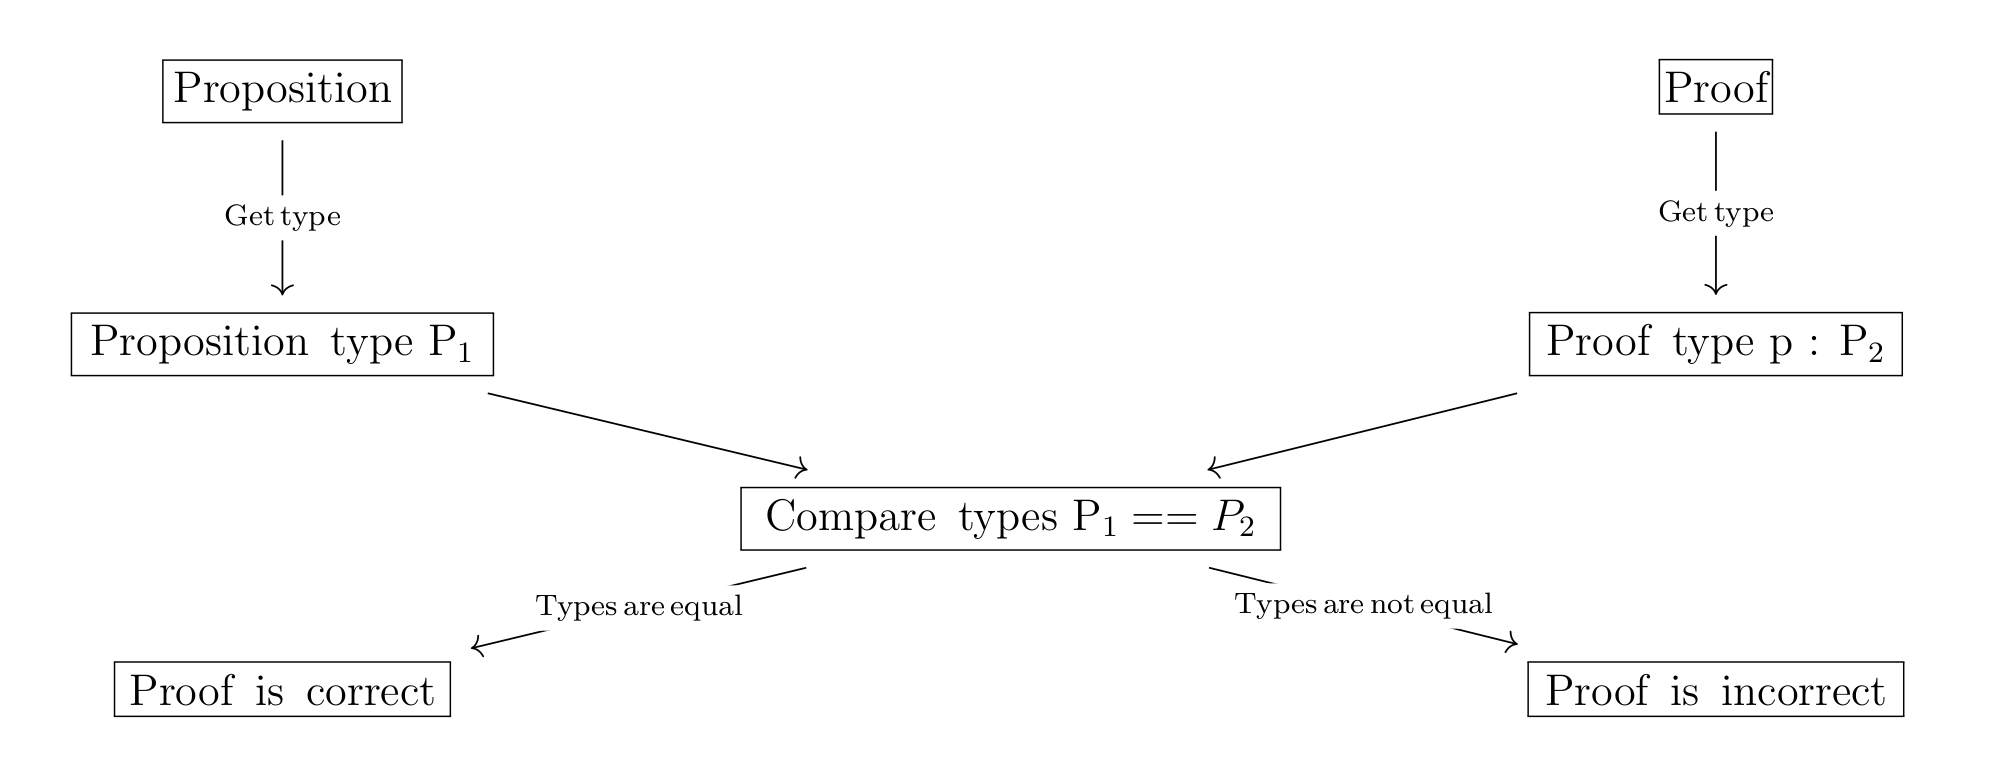
\includegraphics[scale=0.2]{figure1}
\end{center}
\begin{center}
    \scriptsize
    Figure 1: A diagram of the proof checking procedure  our application will use to verify program correctness.
\end{center}
\qquad To further illustrate the feasibility of this project, there exist many applications, or proof checkers, that have successfully implemented a type system to verify the correctness of a given proof. Some examples include Coq, Microsoft’s Lean, and many more. However, we aim to extend upon these systems to check the correctness of programs, rather than purely mathematical proofs.


\section*{Project Components}

\qquad To successfully implement an application that can verify program correctness, major components of our project include a user interface, a scripting language capable of encoding logic, a semantic analysis of a target programming language, a dependent type system, and proof checking algorithms. \\

\noindent \qquad For the user interface, our current idea consists of a text editor where the user may enter program code and a program description. Then our application would merely display whether the user-inputted program performs as the user desires. We would like to expand and improve the user interface, such as by displaying more information and potential visualizations to the user. We will be seeking help from our advisors and conducting more research on how to best visualize such a process. Additionally if time permits, we would consider creating a Visual Studio Code extension or similar. \\

\noindent \qquad An  interpreter is required to parse the program description in order for the application to obtain the type theoretical equivalents of the user input. The description itself will be written in a custom-made scripting language, capable of encoding propositional logic, among other features. Alongside the scripting language interpreter, we require a semantic interpretation of the target programming language. The interpreter will then parse the description as well as the program code so that we may construct the associated type. We are still drafting this process, however it will likely involve the creation of a parse tree, as well as other interpreter-based processes. We seek assistance with creating and implementing such processes.  \\

\noindent \qquad In order to manipulate the types arising from the program description and program code, we require an implementation of a dependent type system. Some examples of rudimentary type manipulation would include $\alpha$-conversion, $\beta$-reduction, abstraction, and application. In order to properly capture the types depicting user input, we will likely require dependent types such as $\Sigma$ and $\Pi$ types to encode quantifiers in logic and iterative control flow statements, as an example. For advisors with mathematical experience, we may ask for guidance in the use of type theoretical constructs. \\

\noindent \qquad Lastly, we will implement proof checking algorithms tailored to our goal of program correctness. As illustrated in Figure 1, we require the use of a “get type” algorithm which will extract the type of the user input after semantic analysis. Additionally, we seek a process of determining whether types are equal.

\section*{Advisor Expectations}

\qquad This is a year-long project, beginning this Fall semester until May of 2022. We need advisors who will be able to commit to us and the project for the entire duration of this project. Advisors will help supervise and provide help and their expertise for our project. This means that advisors must commit to meeting with the team regularly (in-person or online) and dedicate some of their time to the team, which will be determined in a meeting with the team and interested advisors. However, we understand that advisors will only serve as guidance and we will commit to doing the research and coding independently. Additionally, we may seek the advisors’ help on potentially publishing a paper on this project, as much research will be done. Given that this project involves concepts from mathematics and computer science, we wish to have two different advisors with expertise in compilation and type theory, respectively.


\section*{Current Project Progress}

\qquad Currently, we have yet to begin the project. Our proposal was approved for our capstone project on October 12th. However, team members have begun conducting research into understanding how type theory can be applied for program correctness.


\section*{Contact Information}

\qquad Please contact us or the Senior Project Management Team if you have interest in our project or have any questions or concerns. \\

\noindent Diane Du - Computer Sci and Engr BS, Discrete Math BS - dianedu@nevada.unr.edu \\
Landon Fox - Computer Sci and Engr BS, Discrete Math BS - landonfox00@gmail.com \\
Jimson Huang - Computer Sci and Engr BS, Statistics BS - jimson@nevada.unr.edu \\
Logan Leavitt - Computer Sci and Engr BS, Discrete Math BS - loganleavitt@nevada.unr.edu \\

\subsubsection*{CS Software Engineering and Senior Capstone Management}
Dr. Sergiu Dascalu, Professor - dascalus@unr.edu \\
Vinh Le, Instructor - vle@unr.edu


\end{document}

